\let\negmedspace\undefined
\let\negthickspace\undefined
%\RequirePackage{amsmath}
\documentclass[journal,12pt,twocolumn]{IEEEtran}
%
% \usepackage{setspace}
\usepackage{textcomp, gensymb}
%\doublespacing
 \usepackage{polynom}
%\singlespacing
%\usepackage{silence}
%Disable all warnings issued by latex starting with "You have..."
%\usepackage{graphicx}
\usepackage{amssymb}
%\usepackage{relsize}
\usepackage[cmex10]{amsmath}
%\usepackage{amsthm}
%\interdisplaylinepenalty=2500
%\savesymbol{iint}
%\usepackage{txfonts}
%\restoresymbol{TXF}{iint}
%\usepackage{wasysym}
\usepackage{amsthm}
%\usepackage{pifont}
%\usepackage{iithtlc}
% \usepackage{mathrsfs}
% \usepackage{txfonts}
 \usepackage{stfloats}
% \usepackage{steinmetz}
 \usepackage{bm}
% \usepackage{cite}
% \usepackage{cases}
% \usepackage{subfig}
%\usepackage{xtab}
\usepackage{longtable}
%\usepackage{multirow}
%\usepackage{algorithm}
%\usepackage{algpseudocode}
\usepackage{enumitem}
 \usepackage{mathtools}
 \usepackage{tikz}
% \usepackage{circuitikz}
% \usepackage{verbatim}
%\usepackage{tfrupee}
\usepackage[breaklinks=true]{hyperref}
%\usepackage{stmaryrd}
%\usepackage{tkz-euclide} % loads  TikZ and tkz-base
%\usetkzobj{all}
\usepackage{listings}
    \usepackage{color}                                            %%
    \usepackage{array}                                            %%
    \usepackage{longtable}                                        %%
    \usepackage{calc}                                             %%
    \usepackage{multirow}                                         %%
    \usepackage{hhline}                                           %%
    \usepackage{ifthen}                                           %%
  %optionally (for landscape tables embedded in another document): %%
    \usepackage{lscape}     
% \usepackage{multicol}
% \usepackage{chngcntr}
%\usepackage{enumerate}
\usepackage{tfrupee}

%\usepackage{wasysym}
%\newcounter{MYtempeqncnt}
\DeclareMathOperator*{\Res}{Res}
\DeclareMathOperator*{\equals}{=}
%\renewcommand{\baselinestretch}{2}
%\renewcommand\thesection{\arabic{section}}
%\renewcommand\thesubsection{\thesection.\arabic{subsection}}
%\renewcommand\thesubsubsection{\thesubsection.\arabic{subsubsection}}

%\renewcommand\thesectiondis{\arabic{section}}
%\renewcommand\thesubsectiondis{\thesectiondis.\arabic{subsection}}
%\renewcommand\thesubsubsectiondis{\thesubsectiondis.\arabic{subsubsection}}

% correct bad hyphenation here
\hyphenation{op-tical net-works semi-conduc-tor}
\def\inputGnumericTable{}                                 %%

\lstset{
%language=C,
frame=single, 
breaklines=true,
columns=fullflexible
}
%\lstset{
%language=tex,
%frame=single, 
%breaklines=true
%}
\begin{document}

%


\newtheorem{theorem}{Theorem}[section]
\newtheorem{problem}{Problem}
\newtheorem{proposition}{Proposition}[section]
\newtheorem{lemma}{Lemma}[section]
\newtheorem{corollary}[theorem]{Corollary}
\newtheorem{example}{Example}[section]
\newtheorem{definition}[problem]{Definition}
%\newtheorem{thm}{Theorem}[section] 
%\newtheorem{defn}[thm]{Definition}
%\newtheorem{algorithm}{Algorithm}[section]
%\newtheorem{cor}{Corollary}
\newcommand{\BEQA}{\begin{eqnarray}}
\newcommand{\EEQA}{\end{eqnarray}}
\newcommand{\define}{\stackrel{\triangle}{=}}
\newcommand*\circled[1]{\tikz[baseline=(char.base)]{
    \node[shape=circle,draw,inner sep=2pt] (char) {#1};}}
\bibliographystyle{IEEEtran}
%\bibliographystyle{ieeetr}
\providecommand{\mbf}{\mathbf}
\providecommand{\pr}[1]{\ensuremath{\Pr\left(#1\right)}}
\providecommand{\qfunc}[1]{\ensuremath{Q\left(#1\right)}}
\providecommand{\sbrak}[1]{\ensuremath{{}\left[#1\right]}}
\providecommand{\lsbrak}[1]{\ensuremath{{}\left[#1\right.}}
\providecommand{\rsbrak}[1]{\ensuremath{{}\left.#1\right]}}
\providecommand{\brak}[1]{\ensuremath{\left(#1\right)}}
\providecommand{\lbrak}[1]{\ensuremath{\left(#1\right.}}
\providecommand{\rbrak}[1]{\ensuremath{\left.#1\right)}}
\providecommand{\cbrak}[1]{\ensuremath{\left\{#1\right\}}}
\providecommand{\lcbrak}[1]{\ensuremath{\left\{#1\right.}}
\providecommand{\rcbrak}[1]{\ensuremath{\left.#1\right\}}}
\theoremstyle{remark}
\newtheorem{rem}{Remark}
\newcommand{\sgn}{\mathop{\mathrm{sgn}}}
\providecommand{\fourier}{\overset{\mathcal{F}}{ \rightleftharpoons}}
%\providecommand{\hilbert}{\overset{\mathcal{H}}{ \rightleftharpoons}}
\providecommand{\system}{\overset{\mathcal{H}}{ \longleftrightarrow}}
	%\newcommand{\solution}[2]{\textbf{Solution:}{#1}}
\newcommand{\solution}{\noindent \textbf{Solution: }}
\newcommand{\cosec}{\,\text{cosec}\,}
\providecommand{\dec}[2]{\ensuremath{\overset{#1}{\underset{#2}{\gtrless}}}}
\newcommand{\myvec}[1]{\ensuremath{\begin{pmatrix}#1\end{pmatrix}}}
\newcommand{\mydet}[1]{\ensuremath{\begin{vmatrix}#1\end{vmatrix}}}
%\numberwithin{equation}{section}
%\numberwithin{figure}{section}
%\numberwithin{table}{section}
%\numberwithin{equation}{subsection}
%\numberwithin{problem}{section}
%\numberwithin{definition}{section}
\makeatletter
\@addtoreset{figure}{problem}
\makeatother
\let\StandardTheFigure\thefigure
\let\vec\mathbf
%\renewcommand{\thefigure}{\theproblem.\arabic{figure}}
%\renewcommand{\thefigure}{\theproblem}
%\setlist[enumerate,1]{before=\renewcommand\theequation{\theenumi.\arabic{equation}}
%\counterwithin{equation}{enumi}
%\renewcommand{\theequation}{\arabic{subsection}.\arabic{equation}}
\def\putbox#1#2#3{\makebox[0in][l]{\makebox[#1][l]{}\raisebox{\baselineskip}[0in][0in]{\raisebox{#2}[0in][0in]{#3}}}}
     \def\rightbox#1{\makebox[0in][r]{#1}}
     \def\centbox#1{\makebox[0in]{#1}}
     \def\topbox#1{\raisebox{-\baselineskip}[0in][0in]{#1}}
     \def\midbox#1{\raisebox{-0.5\baselineskip}[0in][0in]{#1}}
\title{ Assignment 2 }
\author{ Kotikalapudi Karthik (cs21btech11030)% <-this % stops a space
}
\maketitle
\textbf{ICSE class 12 2018}\\
\textbf{Question 5(b)}\\
Verify Rolle's theorem for the following function:\\
$f(x) = e^{-x} \sin x$ on $\sbrak{0,\pi}$\\
\solution
Given, $f(x) = e^{-x} \sin x$ on $[0,\pi]$\\
For the function to satisfy the Rolle's theorem, the following conditions should be satisfied:
\begin{enumerate}
    \item $f(x)$ should be continuous in $\sbrak{0,\pi}$
    \item $f(0) = f(\pi) = 0$
    \item $f(x)$ should be differentiable in $\brak{0,\pi}$
\end{enumerate}
Here, $e^{-x}$ is an exponential and continuous function and $\sin x$ is a trigonometric and continuous function\\
$\therefore f(x) = e^{-x} \sin x$ is continuous on $\sbrak{0,\pi}$.\\
Also,
\begin{align}
    f(0) &= e^{0} \sin 0 = 0\\
    f(\pi) &= e^{\pi} \sin \pi = 0\\
    \therefore f(0) &= f(\pi) = 0
\end{align}
$f(x)$ is differentiable on $\brak{0,\pi}$ if Left hand derivative(LHD) and right hand derivative(RHD) exists and equal for every $x \in \brak{0,\pi}$ as we already know $f(x)$ is continuous.\\
If $c \in \brak{0,\pi}$, then
\begin{align}
    \text{LHD} &= \lim_{h \to 0^{-}} \frac{f(c+h)-f(c)}{h}\\
    &= \lim_{h \to 0^{-}} \frac{e^{-\brak{c+h}} \sin \brak{c+h} - e^{-c} \sin c}{h}\\
    \label{eq-1}
    &= e^{-c} \lim_{h \to 0^{-}} \brak {\frac{e^{-h} \sin \brak{c+h} - \sin c}{h}}
\end{align}
Similarly,
\begin{align}
    \text{RHD} &= \lim_{h \to 0^{+}} \frac{f(c+h)-f(c)}{h}\\
    &= \lim_{h \to 0^{+}} \frac{e^{-\brak{c+h}} \sin \brak{c+h} - e^{-c} \sin c}{h}\\
    \label{eq-2}
    &= e^{-c} \lim_{h \to 0^{+}} \brak {\frac{e^{-h} \sin \brak{c+h} - \sin c}{h}}
\end{align}
We know that,
\begin{align}
    \label{eq-3}
    \sin \brak{x+h} &= \sin x \cos h + \cos x \sin h\\
    \label{eq-4}
    \text{Also, } \lim_{h \to 0^{-}} \frac{\sin h}{h} &= \lim_{h \to 0^{+}} \frac{\sin h}{h} = 1,\\
    \label{eq-5}
    \lim_{h \to 0^{-}} \cos h &= \lim_{h \to 0^{+}} \cos h = 1,\\
    \label{eq-6}
    \lim_{h \to 0^{-}} e^{-h} &= \lim_{h \to 0^{+}} e^{-h} = 1
\end{align}
From equations \eqref{eq-3} \eqref{eq-4} \eqref{eq-5} \eqref{eq-6}, equation \eqref{eq-1} becomes
\begin{align}
    \text{LHD} &= e^{-c} \lim_{h \to 0^{-}} \brak{e^{-h} \cos c +\frac{e^{-h}sinc - sinc}{h}}\\
    &= e^{-c} \brak{\cos c + \sin c \lim_{h \to 0^{-}} \frac{e^{-h}-1}{h}}
\end{align}
Similarly, from equations \eqref{eq-3} \eqref{eq-4} \eqref{eq-5} \eqref{eq-6}, equation \eqref{eq-2} becomes
\begin{align}
    \text{RHD} &= e^{-c} \lim_{h \to 0^{+}} \brak{e^{-h} \cos c +\frac{e^{-h}sinc - sinc}{h}}\\
    &= e^{-c} \brak{\cos c + \sin c \lim_{h \to 0^{+}} \frac{e^{-h}-1}{h}}
\end{align}
We know that, $\lim_{h \to 0^{-}} \frac{1-e^{-h}}{h}$ and $\lim_{h \to 0^{+}} \frac{1-e^{-h}}{h}$ exist.\\
$\implies$ both LHD and RHD exists.
\begin{align}
    \lim_{h \to 0^{-}} \frac{1-e^{-h}}{h} &= \lim_{h \to 0^{+}} \frac{1-e^{-h}}{h} = 1,\\
    \implies \text{LHD} &= \text{RHD} = e^{-x} \brak{\cos x - \sin x}
\end{align}
$\because$ LHD and RHD exists and equal, we can say that $f(x)$ is differentiable.\\
$\implies f(x)$ is differentiable in $\brak{0,\pi}$.\\
Thus, all the conditions of the Rolle's theorem are satisfied.\\
$\therefore \exists c \in \brak{0, \pi}$ such that $f^\prime(c) = 0$.\\
By differentiating $f(x)$, 
\begin{align}
    \label{eq-diff}
    f^\prime (x) = e^{-x}\brak{\cos x - \sin x}
\end{align}
$\because f^\prime(c) = 0$, substituing $f^\prime(x)$ at $x=c$ from equation \eqref{eq-diff},
\begin{align}
    e^{-c} \brak{\cos c - \sin c} &= 0
    \\
    \implies \cos c - \sin c &= 0
    \\
    \implies c &= \frac{\pi}{4}
\end{align}
Clearly, $\frac{\pi}{4} \in (0,\pi)$\\
Hence, Rolle's theorem is verified.\\
Also, we can see from the graph clearly that all the necessary conditions for Rolle's theorem are satisfied and $f^\prime(\frac{\pi}{4}) = 0$
\begin{figure}[ht!]
	  \centering 
	  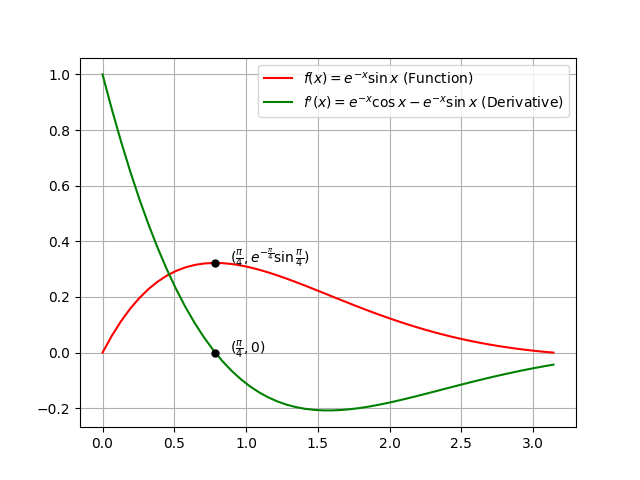
\includegraphics[width=\columnwidth]{Figs/Figure_1.png}
	  \caption{Graph of $f(x)$ and $f^\prime(x)$ in $\sbrak{0,\pi}$}
	  \label{fig-1}
\end{figure}

\end{document}
